\documentclass{article}
\usepackage[utf8]{inputenc}

\usepackage{tikz}
\usetikzlibrary{positioning, fit}

\usepackage{skak}

\begin{document}

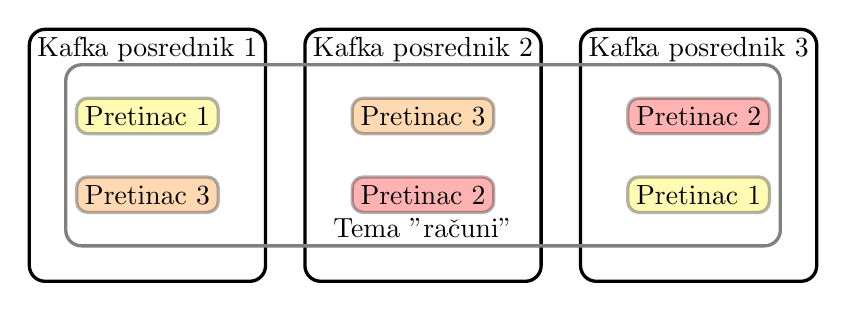
\begin{tikzpicture}[ % has a lot of options; consult the pgf manual
bend angle=45,
long_square/.style={rectangle, draw=black, fill=white, very thick, inner sep=3pt, minimum width=14mm},
rounded_square/.style={rectangle, rounded corners, draw=black, fill=white, very thick, inner sep=3pt, minimum width=14mm},
empty_circle/.style={rectangle, rounded corners=2mm, draw=black, fill=white, very thick, minimum size=4mm},
point/.style={circle, inner sep=0mm},
fit_square/.style={rectangle, rounded corners=2mm, draw=black, very thick, minimum height=32mm, minimum width=30mm},
both_arrow/.style={<->, very thick},
out_arrow/.style={->, very thick},
in_arrow/.style={<-, very thick},
above_edge_text/.style={above, midway, sloped}
]

\node[rounded_square, fill=yellow, opacity=0.3, text opacity=1.0](leader_1) at (0,0) {\king Pretinac 1};
\node[rounded_square, fill=orange, opacity=0.3, text opacity=1.0](leader_3) at (3.5,0) {\king Pretinac 3};
\node[rounded_square, fill=red, opacity=0.3, text opacity=1.0](leader_2) at (7,0) {\king Pretinac 2};

\node[rounded_square, fill=orange, opacity=0.3, text opacity=1.0](follower_3) at (0,-1) {\pawn Pretinac 3};
\node[rounded_square, fill=red, opacity=0.3, text opacity=1.0](follower_2) at (3.5,-1) {\pawn Pretinac 2};
\node[rounded_square, fill=yellow, opacity=0.3, text opacity=1.0](follower_1) at (7,-1) {\pawn Pretinac 1};

\node[fit_square, fit=(leader_1) (follower_3)] (broker_1) {};
\node[anchor=north] at (broker_1.north) {Kafka posrednik 1};

\node[fit_square, fit=(leader_3) (follower_2)] (broker_2) {};
\node[anchor=north] at (broker_2.north) {Kafka posrednik 2};

\node[fit_square, fit=(leader_2) (follower_1)] (broker_3) {};
\node[anchor=north] at (broker_3.north) {Kafka posrednik 3};

\node[rounded corners=2mm, draw=gray, very thick, minimum height=23mm, fit=(leader_1) (leader_2) (leader_3) (follower_1) (follower_2) (follower_3)] (topic) {};
\node[anchor=south] at (topic.south) {Tema "računi"};

\end{tikzpicture}

\end{document}